

\chapter{Neuaufbau des Vorgängerprojekts}

Im Kapitel 2 werden die Beweggründe für einen Neuaufbau dieses Projektes erläutert.




\section{Historie der entstandenen Probleme}

Das Projekt wurde schon von mehreren Gruppen in der Vergangenheit bearbeitet. Dabei hat jede Gruppe die Probleme der vorherigen Gruppe aufgefasst und versucht zu lösen. 

\subsection*{1. Gruppe:} 

Das ursprüngliche Ziel war es das Fahrzeug einen Raum zu Kartographieren und die Lokalisierung an einem externen PC darzustellen. Dazu wurde ein Raspberry Pi als Steuereinheit verwendet. Der Lidar wurde über das ROS-Framework angesprochen und die ROS-Daten via WLAN an einen externen PC gesendet. Der externe PC stellte die Karte mit RViz dar.

\subsection*{2. Gruppe:} 

\textbf{Problem}: Das Framework \acrfull{ros} benötigt zu viele Ressourcen auf dem Raspberry Pi A\\
\textbf{Lösung}: ROS entfernen und die Rohdaten über einen Socket manuell an externen PC senden. Externer PC baut die Rohdaten wieder zu ROS-Daten zusammen und stellt die Karte mit RViz dar.

\subsection*{3. Gruppe:} 

\textbf{Problem}: Raspberry Pi A ohne ROS immer noch zu langsam, um die Daten schnell genug an externen PC weiterzusenden.\\
\textbf{Lösung}: Den Raspberry A entfernen. Neuer Aufbau:

\begin{itemize}
\item Ein \acrfull{fpga} (NIOSII) mit dem Betriebssystem FreeRTOS zur Kommunikation (über SPI, I2C) verwenden.

\item Die Hardware (Lidar, Ultraschallsensoren, Licht, etc.) geben Daten direkt an das FPGA, welches die Daten dann weitersendet.

\item \acrfull{hps} hat eigenes Linux auf interner SD-Karte, spricht FPGA (über Shared Memory) an und sendet Daten über WLAN an externen PC.
\end{itemize}




\subsection*{4. Gruppe:} 

\textbf{Problem}: kein autonomes Fahren möglich, keine Karte wurde erstellt\\
\textbf{Lösung}: Lidar übergibt HPS Rohdaten, HPS führt SLAM aus und erstellt Karte. Die erstellte Karte wird an externen PC gesendet und dort dargestellt. Echtzeitverhalten des HPS soll durch angepasste Auslastung erreicht werden.


\section{Vorhandene Probleme beim Projektstart}


Nach der 4. Gruppe traten folgende Probleme auf:

\subsection*{Probleme an der Hardware}

\begin{itemize}
\item  Hardware liefert keine zuverlässigen Odometriewerte
\item  SLAM verwendet keine Odometrie (Probleme insbesondere bei 180° Drehungen)
%\item  Verbesserung des SLAM ohne Odometrie durch (Durchschnitts-Geschwindigkeit, Rad-Rotary-Encoder, MPU Beschleunigung und Rotationswerte) lieferten keine Verbesserungen der Karte.
\item Regelmäßiger Ausfall des Motortreibers
\end{itemize}







%\section{Probleme an der Hardware}

%- die Daten der MPU gehen irgendwo auf dem Weg zwischen Sensor - FPGA - NIOS2 - Netzwerksocket - Empfang beim ext. Rechner verloren
%- laut Dokumentation der Vorgängergruppe ist es hardwarebedingt nicht möglich die Beschleunigungswerte in die Verarbeitung durch den SLAM mit einzubeziehen (genauere Infos dazu haben wir nicht gefunden)
%- der Motortreiber stürzt immer häufiger ab, sodass ein Testen aktuell so gut wie nicht mehr möglich ist
%- die Ultraschallsensoren werden nicht ausgewertet
%- der Hardware- sowie Softwareaufbau erscheint recht kompliziert, sodass viel Zeit für die Einarbeitung benötigt wird



\subsection*{Probleme an der Software}

\begin{itemize}
\item Da es viele Stationen zwischen Sensor und Darstellung auf externem PC gab, waren mögliche Fehler auf den Zwischenmodulen (FPGA, NIOS2, Netzwerksocket) nur sehr schwierig auszumachen.

\item Die Dokumentation über den bisherigen Aufbau in den Bereichen Hardware, Einstellungen des Betriebssystems sowie am vorhandenen Quellcode waren sehr unzureichend und es war extrem schwierig darauf aufzubauen. 

\end{itemize}

Nach einer längeren Einarbeitungszeit, in der die Module und der Projektverlauf aufgearbeitet wurde, war die einzig sinnvolle Entscheidung die gesamte Hardware sowie Software zu überarbeiten. Dabei wurde Wert auf die Trennung der Module und die Übersichtlichkeit gelegt. 


\section{Aktueller Aufbau des Autonomen Laser Fahrzeugs (Alf)}

In Abbildung \ref{fig:alf_new} ist der neue und verbesserte Aufbau des ALF ersichtlich. 


% Aufbau einer SLAM karte
% Wegefindung mit Djikstra
% Bewegungssteuerung 
% 3 hauptmodule



\begin{figure}[hbtp]
\centering
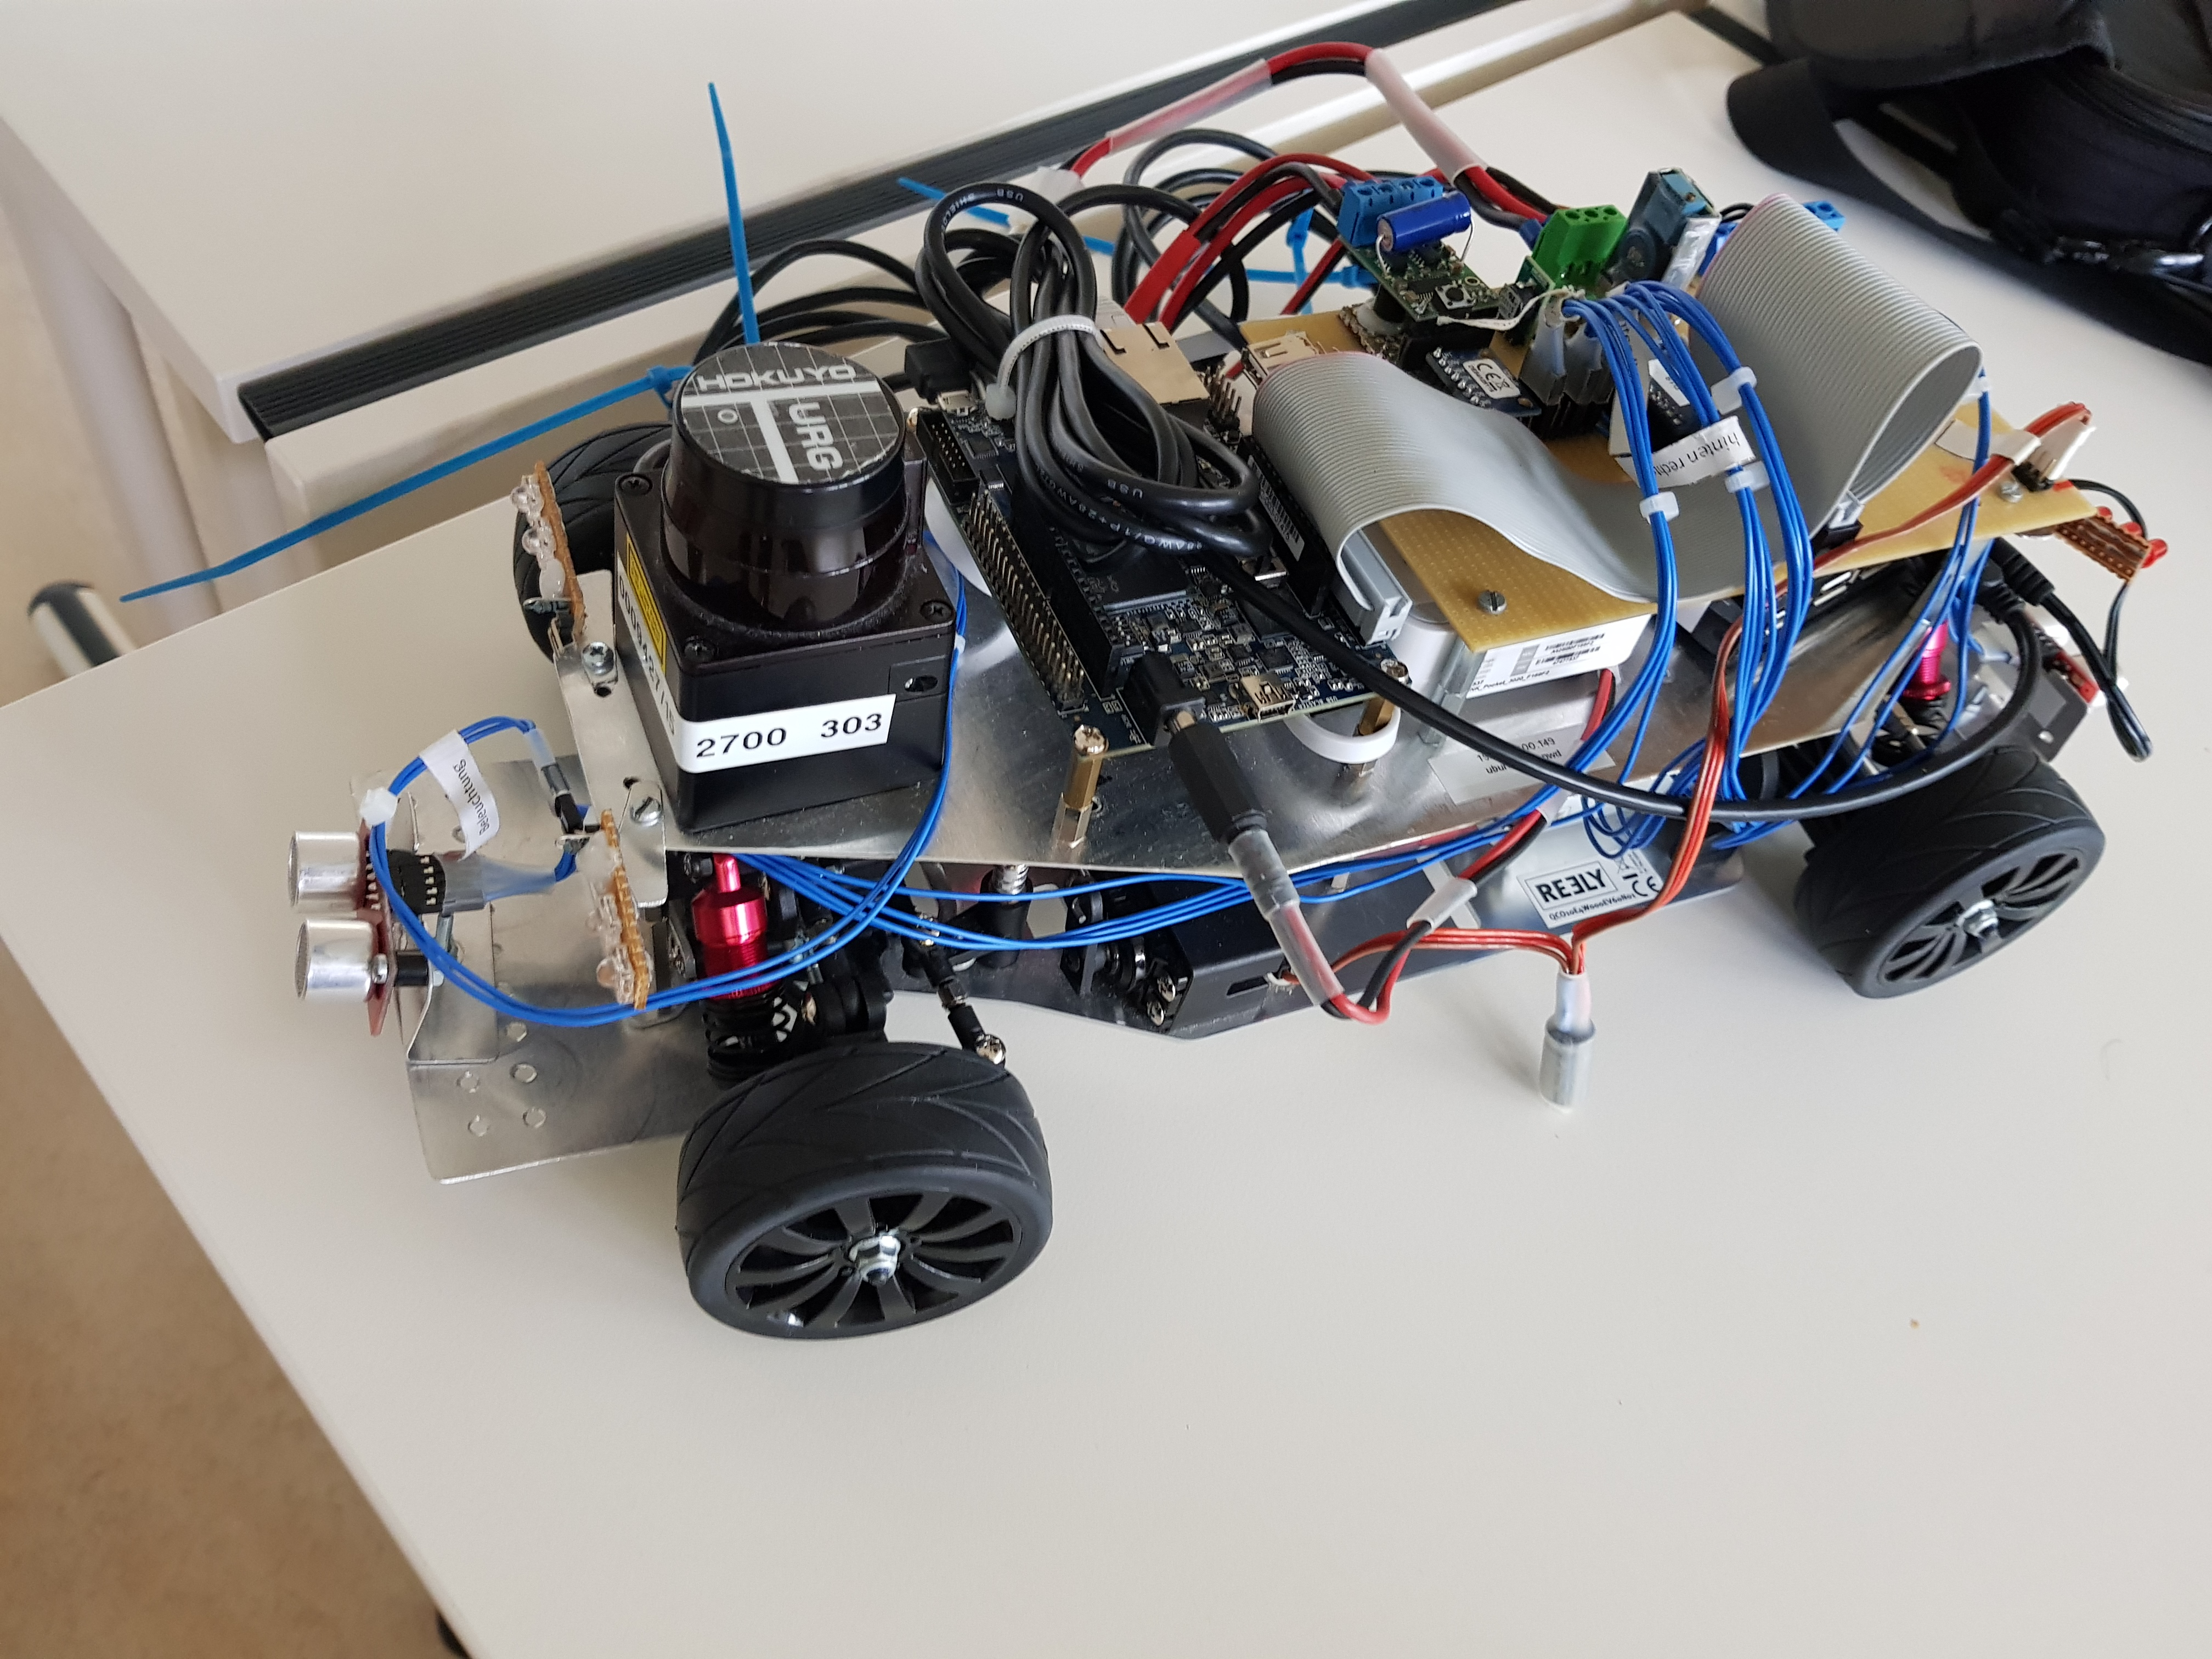
\includegraphics[scale=0.1]{images/chapter2/alf_old.jpg}
\caption{Aktueller Aufbau des ALF}
\label{fig:alf_new}
\end{figure}